\RequirePackage[T1]{fontenc}
\documentclass[conference,10pt]{IEEEtran}
\usepackage{amsmath,amssymb,graphicx,url}
\title{Current-STA Transactional Repair for Timing--Resource Tradeoffs in 3D FPGA Routing}
\author{\IEEEauthorblockN{Anonymous development manuscript}}
\begin{document}
\maketitle
\begin{abstract}
Legal FPGA routes trade timing, wire and vertical resources. Our current-STA repair searches connection groups on private trees and commits after physical, capacity and native timing checks. Retained-crossing domains encourage sharing; search failure releases the affected network's domain. Three timing repairs improve strong native BNN from 13.607436 to 13.228146 ns for forty extra wire units. From identical fresh roots, native/domain-first flows take 7933.25/9754.31 s at equal final CPD; domain-first spends 1786 wire for 39 fewer SB/two fewer CB, attaining a fixed-terminal vertical bound. Matched owner-scope repairs escape a certified single-net local minimum with unchanged endpoint vectors. Separate fixed-input feedback improves ten setup components without regressions. Fixed-input controls expose grouping, timing-budget and acceptance-scheduling tradeoffs. Robot transfer saves one CB for 20 wire; a distinct constrained robot input has no applicable sharing cut or accepted timing repair. Conv-layer and attention pairs fail initial routing. Single-pass indexing preserves BNN execution at 7463.17 s. Mechanism ablations separate sharing domains, failed-search release and owner coordination. A prospective fixed-version conv-hls pair retains its root; positive integrated confirmation remains pending.
\end{abstract}
\begin{IEEEkeywords}
3D FPGA, detailed routing, static timing analysis, transactional repair, multiobjective optimization
\end{IEEEkeywords}

\section{Problem and Motivation}
Three-dimensional FPGA routing couples directed reachability, scarce vertical channels and timing. With packing, placement and architecture fixed, repair may improve CPD or trade resources under an explicit timing requirement. Shorter local connections need not improve the complete route: another endpoint may become critical or capacity may block another network.

VTR supplies routing and STA infrastructure~\cite{vtr9paper}; LaZagna models configurable vertical SB/CB architectures~\cite{lazagna}, while Escaping Flatland improves 3D placement~\cite{flatland}. We hold architecture, packing and placement fixed. Reduced resource occupancy does not imply silicon-area or power savings.

PathFinder negotiates congestion using timing priorities~\cite{pathfinder}. Critical-connection repair after PathFinder predates this work~\cite{liurepair}. AIR preserves legal subtrees, reroutes illegal or delay-degraded connections, and improves existing routes through multiple convergences~\cite{air}. CRoute uses timing-driven connection-based routing~\cite{croute}. Current timing, retained trees and incremental rerouting are therefore established ingredients. Our comparison concerns conditional vertical sharing domains, per-net domain release and capacity-certified owner scopes, with whole-candidate acceptance under fixed timing/resource envelopes. We do not claim a new native router or measured superiority over these external implementations.

Poolad et al. introduce explicit CHANZ resources and multi-die-aware lookahead~\cite{multidie}. Our edge-encoded two-layer results do not validate those architectures or their lookahead. The contributions supported here are matched local mechanism effects, complete resource/time tradeoffs and explicit failure/applicability accounting. The fully integrated frozen controller remains a confirmation target.
\section{Method: Current-State Transactional Repair}
\subsection{Objectives and state identity}
An input identity fixes the directed resource graph, packed netlist, placement, endpoint mapping, SDC and clock domains. A legal route $R$ uses actual graph edges and respects node capacities and native routing constraints. We record
\begin{equation}
 q(R)=(D(R),W(R),S(R),C(R),T(R)),
\end{equation}
where $D$ is native final CPD, $W$ is planar wire in the auditor's native resource units, $S$ is occupied SB pairs, $C$ is occupied CB output sources, and $T$ is comparable complete algorithm time. Paired SB half-nodes are one vertical resource; multiple CB edges from one output are not independent outputs. Guide recommendations are not occupancy measurements.

Nondominated archives bind versions and opportunities. Quality projections cannot establish quality/time dominance when complete cost is unknown.

Final retention is separate from a branch's transition rule. We retain a strict CPD mode, $D(R')<D(R)$, and a fixed-resource mode that reduces CPD within registered absolute resource limits. A resource-under-timing mode permits wire tradeoffs within a fixed envelope while requiring nonincreasing selected resource objectives and at least one strict reduction. The current resource probes select $(S,C)$ as those objectives, cap CPD at the root value, cap wire at the root value plus 0.1\%, and prohibit increases beyond root vertical counts. A separate experiment fixes CPD at 102\% of the initial root once. These design parameters do not define research termination.

Endpoint-vector acceptance fixes endpoint/launch/capture identities and requires nonworse CPD, nonworse setup components, one strict setup improvement and no increased hold violation. Native comparisons use no epsilon. Resource policies apply their stated CPD/hold constraints; bounded vector additionally enforces the strict control's fixed wire/SB/CB caps. Anchors never roll forward.


\subsection{Select targets and dependency scopes}
Timing selection follows current native winning paths, including tied fan-ins. Capacity queries identify blocking owners; grouped targets and owner scopes release dependencies frozen by single-connection repair.

Resource selection scans the actual current route trees. A candidate removes all sinks below a selected crossing subtree, preserves paths to the other sinks, and requires both structural release potential and a retained crossing alternative. The screen uses current slack margin; it is not a proof of final resource savings. Ranking is deterministic: released crossings per removed sink, fewer sinks, larger current margin, then network and pin IDs. A K 8 group contains at most eight distinct networks; fewer are used when fewer qualify. Removed connections are restored in descending current raw criticality with deterministic ties. Accepted states receive a fresh current selector.

A diagnostic selector escalates stalled source escapes. When a SOURCE's sole OPIN has unit-capacity same-layer channel exits all held by others, a same-layer sink forces an outward crossing and a distinct return resource. Owner-descendant cuts are screened by current STA and ranked by crossing excess, connection count, margins and IDs. Complete native checks still determine feasibility.

\subsection{Native searches and retained-crossing domains}
For each group we copy the selected trees and prune exactly the registered sink sets. Occupancy is updated as every local replacement is installed, so later searches see earlier resource use. Native weighted search uses the full device search box and the existing timing/congestion objective. Capacity-infeasible results are not committed. Real switch delays and final STA remain unchanged.

The domain permits cross-layer edges only through sources retained after pruning. The unrestricted control uses the same source, sinks, scope, objective and search range. Development probes evaluate both variants; CP1 tries the domain first and omits the native diagnostic only after complete resource acceptance. Rejection or infeasibility retains same-source native fallback. After divergence, each arm reselects from its own accepted states. Unexecuted candidates have no inferred metrics.

If guided search fails to return a capacity-feasible branch, failure release resets search costs and removes only that network's domain. Prior restorations/occupancy remain private; other networks stay guided. Operational search failure does not certify mathematical infeasibility; a separate capacity diagnosis may establish a fixed-scope bound.

\subsection{Complete checks, acceptance and restoration}
After restoring all selected connections, independent checks validate real edges, retained branches, terminals, global capacity and resource counts; native FULL/fresh STA check the replacement. Acceptance commits the entire group; failure/rejection retains the source. Private intermediate states may spend resources/slack if the complete combination passes, allowing useful groups whose components individually fail CPD improvement.

Candidates receive native LOAD/FULL/STA, or private-worker FULL/fresh STA and export. Worker restoration covers trees, sink lookups, occupancy, digest and hooks before reobservation. Tiny/BNN-resource/free-path timing checks match separate LOAD/STA; large forced-path timing remains unvalidated.

AIR retains historical congestion costs across convergences~\cite{air}; our imported contexts reset PathFinder prices. Matched controls share that reset. In-router continuation requires a separate price-history comparison.


\subsection{Composition and terminal selection}
Construction, transaction acceptance and terminal selection are separate. Private intermediates may spend slack or capacity; only complete checked candidates become observations or commits. The fixed terminal rule selects eligible states from that execution.

\begin{figure}[t]
\centering\footnotesize
\fbox{\begin{minipage}{.93\columnwidth}
\textbf{CP1 fixed controller contract}\\
1. Bind input, binary, root envelope and terminal rule.\\
2. Route; retain initial failure if no legal root exists.\\
3. Observe current STA, trees, capacity and crossings.\\
4. Select current target cuts and a deterministic group.\\
5. If sharing is available, try the retained-crossing domain; on failed search, release only the affected net.\\
6. If a diagnosed owner blocks the relevant escape, construct a separate matched owner-coordination group.\\
7. Check the whole candidate with native FULL/STA, physical edges, retained scope and capacity.\\
8. Archive legal candidates; accept or restore under the fixed policy. Reobserve after each commit.\\
9. On menu closure, apply the fixed terminal rule and report complete cost and all outcome classes.
\end{minipage}}
\caption{Relationship between the mechanisms. CP1 fixes executable source, input interpretation and these rules. Independent complete confirmation and positive integrated branch coverage remain pending. A mechanism branch is not assumed to improve every metric.}
\label{fig:method}
\end{figure}

Crossing redundancy enables sharing; capacity obstruction justifies an owner proposal; current slack screens complete cuts. Failed search triggers local release, not global infeasibility. Scoped owner effects differ: R1 reduces vertical counts, while robot below trades extra resources for endpoint gains. CP1 freezes the core/input contract; CP1r2 adds the runtime corrections below. Outside-project observation, a known R1 owner transaction and an existing tiny whole flow pass; positive automatic owner reentry, positive integrated timing feedback and independent benefits remain unverified. Existing development runs are not retroactively confirmation.
\section{Complete Results and Transfer}
The implementation derives from VTR revision \texttt{0b912334fdd83bb754b302146ac0d1ec9edc9a0e}. Fixed-input serial clustered routing uses two-layer edge-encoded Hybrid-O/SB-only/CB-only graphs, ideal clocks and native FULL/STA. Each record binds physical inputs, constraints, binary, request and acceptance. Flat routing, CHANZ and general multilayer remain unvalidated. A0 is native; R1 is the older guided method. Strong BNN roots permit eight native convergence attempts with a 1.01 threshold. BNN has no supplied SDC: defaults use one ideal ap\_clk domain and zero input/output/setup/hold constraints; bound echoes fix these. U/Tf remain separate versions/opportunities.

\begin{table*}[t]
\centering\footnotesize\setlength{\tabcolsep}{3 pt}
\caption{Unified complete attempts and scoped ablations. Grouped infrastructure rows report cost/PSS ranges; per-arm receipts are supplementary. N/D: native/domain-first. Hybrid-O except eltwise alternate-topology rows; router seed 11. Robot SDC: distinct placement, 20-ns clock, 1/0-ns maximum/minimum I/O. SB 102\% caps CPD at 1.02 times root. PSS: sampled tree sum, GiB. Endpoints: improved/regressed setup and increased hold violations versus each arm's own root. $^{*}$GNU-time, 1-s precision; observer/PSS lost, brief overlap. $^{\dagger}$Imported scope only. $^{\ddagger}$Owner-minus-target deltas; shared pair cost/PSS.}
\label{tab:completecost}
\begin{tabular}{lrrrrr}\hline
Circuit/role & CPD(ns) & Wire/SB/CB & Time(s) & PSS & Setup $+/-$/Hold$^-$\\\hline
Eltwise N&6.018101&217050/26/968&290.19&1.274&23/2/0\\
Eltwise D&6.018101&217183/24/965&289.21&1.302&26/25/0\\
SPMV N&7.034698&148463/0/967&91.69&1.010&0/0/0\\
SPMV D&7.034698&148463/0/967&91.55&1.034&0/0/0\\
Softmax N&8.975747&169486/3/713&274.22&2.502&29/0/0\\
Softmax D&8.975747&169486/3/713&336.68&2.534&29/0/0\\
SB-only N&6.040485&227439/999/0&424.59&1.271&2/49/0\\
SB-only D&6.040485&227459/999/0&533.57&1.282&0/27/0\\
CB-only N&5.862299&212511/0/982&74.15&0.740&0/0/0\\
CB-only D&5.862299&212511/0/982&72.46&0.740&0/0/0\\
SB 102\% N&6.040485&227439/999/0&448.09&1.285&2/49/0\\
SB 102\% D&6.114032&227583/995/0&581.65&1.257&90/482/0\\
BNN cold N&13.228146&2059631/82/5062&7933.25&11.055&14/17/0\\
BNN cold D&13.228146&2061417/43/5060&9754.31&11.063&547/820/0\\
BNN index N&13.228146&2059631/82/5062&7463.17&11.062&14/17/0\\
BNN stream N&13.228146&2059631/82/5062&7247$^{*}$&--&14/17/0\\
BNN stream D&13.228146&2061417/43/5060&9116.40&11.067&547/820/0\\
Robot N&13.354624&251116/9/653&377.71&2.517&209/0/0\\
Robot D&13.354624&251136/9/652&424.45&2.509&209/32/0\\
Conv-layer N (initial fail)&--&--&260.10&--&--\\
Conv-layer D (initial fail)&--&--&254.57&--&--\\
Eltwise lazy+snapshot D&6.018101&217183/24/965&198.88&1.274&26/25/0\\
Softmax lazy+snapshot D&8.975747&169486/3/713&256.54&2.456&29/0/0\\\hline
BNN terminal N&13.228146&2059607/82/5062&7351.26&11.063&16/17/0\\
Robot SDC N&12.727250&250411/2/526&498.00&2.438&0/0/0\\
Robot SDC D&12.727250&250411/2/526&504.09&2.421&0/0/0\\
Attention N (initial fail)&--&--&794.67&--&--\\
Attention D (initial fail)&--&--&792.69&--&--\\\hline
CLSTM N (load fail)&--&--&107.00&0.450&--\\
CLSTM D (load fail)&--&--&106.48&0.450&--\\
Robot p1 N (load fail)&--&--&102.93&0.451&--\\
Robot p1 D (load fail)&--&--&102.90&0.451&--\\\hline
Conv-hls CP1r2 N&14.351002&84291/0/37&505.17&3.964&0/0/0\\
Conv-hls CP1r2 D&14.351002&84291/0/37&500.90&3.964&0/0/0\\
Supervision interrupted (5 arms)&--&--&346.66--6147.85&2.639--10.927&--\\
Guard launch failed (4 arms)&--&--&103.04--185.03&0.452--0.666&--\\
\hline
\multicolumn{6}{l}{Fixed imported-scope components (not complete configurations)}\\

Robot no-release$^{\dagger}$ (rollback)&--&--&29.24&--&--\\
Robot owner $\Delta^{\ddagger}$&0&+12/0/+1&155.10&2.340&31/0/0\\\hline
\end{tabular}
\end{table*}


Table~\ref{tab:completecost} retains 34 complete attempts (four routing and four loading failures), five supervision-interrupted and four pre-native launch failures (two grouped rows), and two scoped components; the owner row reports paired deltas and shared cost. The measurement starts from supplied architecture, RR graph, BLIF, packed netlist and placement, includes index construction, fresh routing, complete repair, actual rejected candidates, native STA, checks and rollback, and ends at the final seal. Packing, placement and compilation are upstream. BNN resource and timing phases use explicitly bound different binaries. The other full-flow rows are complete resource-repair configurations; identical notation does not imply identical portfolios across rows.

The original complete BNN native/domain pair starts with identical route trees and endpoint vectors. Native makes five resource commits, domain nine; both then make three current-STA timing commits and reach 13.228145690 ns. Domain uses 2061417 wire,43 SB,5060 CB against native 2059631,82,5062. It spends 1786 wire and 1821.07 s (22.95\%) for 39 fewer SB and two fewer CB. Setup changes include 534 improvements and 803 regressions, with no increased hold violation: equal CPD is not endpointwise equivalence.

The SB reduction is $(82-43)/82=47.56\%$. The reduction in total counted vertical resources is $(5144-5103)/5144\simeq 0.797\%$. These denominators answer different questions. Saving scarce SB occupancy can matter on a fixed device even when CB dominates the total. It does not reduce fabricated area or establish power or routability improvement on other designs.

Eltwise domain-first trades 133 additional wire for two fewer SB and three fewer CB relative to native at the same CPD. Both SPMV roles retain 148463 wire,zero SB,967 CB with no eligible cut; this is a no-op, not global optimality. Softmax native/domain both reduce six to three SB and four wire units, while domain-first adds one native transaction and 62.46 s with no final quality benefit.

Robot native/domain reach 251116/251136 wire,9/9 SB and 653/652 CB at equal 13.354624073 ns, with 377.71/424.45 s whole cost. Thus domain trades 20 wire and 46.74 s for one CB. Both conv-layer roles fail initial routing within 200 iterations, costing 260.10/254.57 s; no legal quality or repair result exists. This transfer cohort has two successes among four registered roles. Historical directory names containing ``heldout'' do not make these known circuits unseen tests.

The new robot input changes actual placement and supplies an explicit 20-ns clock with maximum/minimum I/O delays of 1/0 ns. Both arms have identical initial route bodies/full vectors and identical final vectors: 12.727250365 ns,250411 wire,2 SB,526 CB. All 10972 observed setup and hold components are finite and nonnegative. This is a declared benchmark target, not an external application requirement. Neither sharing nor owner screening finds an eligible cut; all three timing proposals are rejected. A legal 12.671110383-ns proposal spends eight wire,one SB and one CB beyond the registered resource limits. The fixed rule retains the root at 498.00/504.09 s (descriptive +1.22\%); no mechanism benefit is established. Attention fails initial routing in both arms after 200 iterations with 231 overused nodes, costing 794.67/792.69 s; repair is never entered. These four development roles yield two legal outputs on one known physical input, not two independent successes.

The prospective CP1r2 conv-hls pair has matching initial trees/full vectors and unchanged finals: 14.351002164 ns, 84291 wire, 0 SB, 37 CB, 4491 setup/hold components; zero commits/proposals. All 18 selected connections have zero physical gain with fixed or relaxed capacity, including seven conflicting relaxed witnesses. Costs are 505.17/500.90 s, 3.964/3.964 GiB sampled PSS, 1/4 missing samples. This confirms one fixed-menu no-op input, without global optimality or interleaved speedup.

On the fixed eltwise packing/placement, SB-only native/domain both reach 999 SB under the strict CPD cap; domain uses 20 more wire and 108.98 more seconds. CB-only has no eligible cut, retaining 982 CB sources. Thus applicability depends on actual crossing structure and timing headroom, not simply the presence of a 3D graph. Router seeds 11 and 19 reproduce the same eltwise/softmax roots and trajectories, adding no independent physical starts.
\section{Multiobjective Tradeoffs}
\begin{figure*}[t]
\centering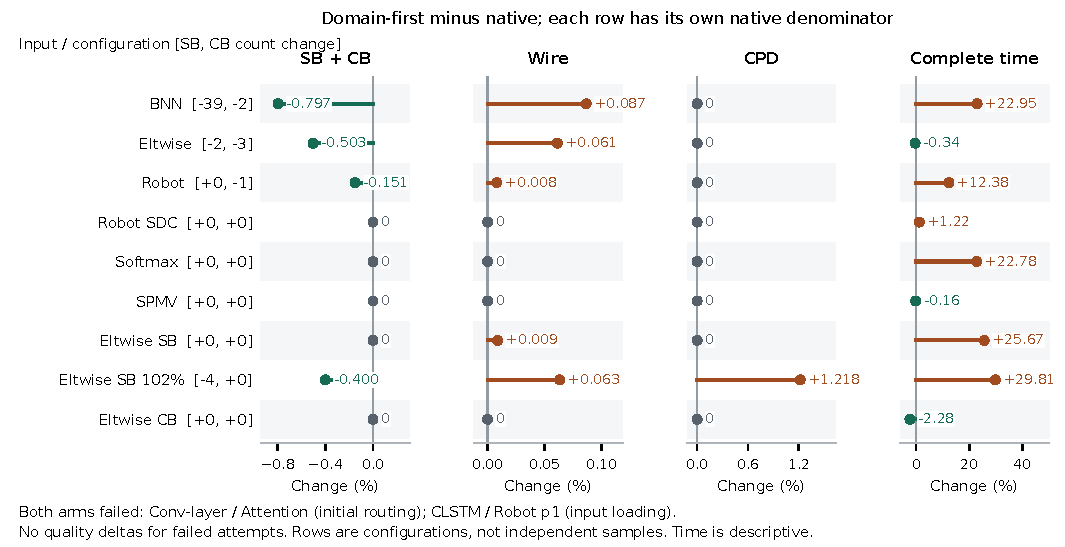
\includegraphics[width=.98\textwidth]{data/complete_paired_tradeoffs_10.pdf}
\caption{Complete domain-first/native tradeoffs from Table~\ref{tab:completecost}: $100(D-N)/N$ within each matched pair. Brackets report separate SB/CB count changes. Each panel has its own scale; lower is better for that metric. Nine development configuration pairs are not nine independent inputs; the new no-op confirmation pair is reported in Table~\ref{tab:completecost}. Initial/input failures and grouped infrastructure failures retain costs without quality deltas. Single-run time differences are descriptive, not statistical speedups.}
\label{fig:joint}
\end{figure*}

The strong native A 0 BNN root is 13.607436067 ns,2059567 wire,94 SB,5062 CB. Three current-STA strict commits reduce CPD by 2.787376\% to 13.228145690 ns for 40 wire units, keeping vertical counts. The third step regresses a noncritical setup component; strict CPD and endpoint-vector rules therefore select different trajectories. Grouped repair can also improve a setup component when its first smaller subgroup is endpoint-flat and rejected. Complete group acceptance is essential to evaluating such combinations.

Complete resource--timing pairs belong in a joint quality/cost comparison. Older imported native/domain endpoints have four/28 fewer wire than the fresh complete pair but lack comparable complete times. They remain quality observations and are not assigned the new cold costs. Figure~\ref{fig:joint} instead compares complete paired outcomes across circuits and configurations, retaining no-gain cases and failures. Historical local projections, dominated/rejected candidates and their full vectors remain in the supplement; coincident points add no independent samples.

Fixed terminal layers require 5103 counted nonglobal networks to cross. The audited graph has unit-capacity CB sources and uniquely paired unit-capacity SB halves. Distinct networks therefore require distinct counted resources: $S+C\ge 5103$. The 43-SB/5060-CB route attains that bound; under $C\le 5060$, $S\ge 43$ is attained. This is fixed-graph vertical occupancy optimality, with no claim of optimal placement, wire or timing.

A fixed timing envelope permits other useful points. On SB-only eltwise, setting the CPD limit once to 102\% of the root allows the domain branch to reach 995 SB,227583 wire and 6.114032 ns, versus native 999 SB,227439 wire and 6.040485 ns. It trades 144 wire,1.218\% CPD and 133.56 s for four fewer SB. The envelope is development-derived, not an external application requirement or unseen-test result.

Final selection is distinct from SB/CB transition acceptance. An existing Tf candidate saves 80 wire at unchanged CPD/SB/CB but changes setup components by 19 improvements/four regressions. A fixed-timing terminal rule accepts it; endpoint nonregression rejects it. The three-net composition passes native FULL/STA: 2059607 wire,82 SB,5062 CB at 13.228145690 ns, saving 24 wire from its source with two setup improvements and no regression; all 34 predicted delays match. Its 217.95 s covers imported validation. A separate complete terminal-selection flow reaches the same scalar quality in 7351.26 s, including fresh routing, indexes, rejected proposals and three timing commits. The separate audit confirms identical resource-prefix states, requests and native work, with 24 fewer final wire and two setup improvements without regression. Matched GNU-time is 7351/7247 s (+104 s); the old observer/PSS loss and overlap remain. This same-input tradeoff is not acceleration.
\section{Mechanism Ablations and Attribution}
\subsection{Domain restriction and failure release}
Domain restriction encourages cross-layer reuse under a fixed cut. Its contribution is evaluated against an unrestricted search from the same source, request, seed, scope and objective. After trajectories diverge, native and domain controls select from their own current successors. Eltwise and softmax never trigger failed-search release: their results cannot be credited to that mechanism. Softmax's equal final quality and SB-only's unfavorable strict-budget result remain negative evidence for universal domain benefit.

In an R1 transaction, a guided net fails after five restorations. Capacity reachability is absent both immediately after pruning and at failure, whereas unrestricted search has a witness. This proves a fixed-scope/domain obstruction, not global unroutability.

Automatic release of only the failed network reproduces the selective-release route and full endpoint vector. It reaches 72 SB versus 74 for the matched unrestricted control, at 64 more wire and unchanged CPD/CB. Nine setup components improve with no regression; strict CPD rejects but endpoint-vector acceptance succeeds. Release preserves guidance for other networks, so its benefit must be separated from disabling all domains.

In robot's first matched transaction, a still-guided net saves one CB; two nets release their domains. A source-cut audit separates the mechanisms: every same-layer source exit is held at unit capacity by an owner outside the transaction, while the retained domain allows only outward crossing sources. A source-layer sink cannot return under that domain. Release removes this domain obstruction, but both actual candidates retain two crossings per blocked net; freeing outside owners is a separate intervention. Disabling only release in the same 23-connection transaction fails on its first connection after nine attempts; source bytes and the full endpoint vector are restored exactly. This native ablation supports release as an operational enabler. The cut audit establishes the conditional obstruction; the matched owner test below separates coordination.

\subsection{Blocking-owner coordination}
R 1's remaining excess crossing exposes a different limitation: all eight same-layer OPIN exits are owned by other nets. Fixed-scope trials preserve the extra crossing or fail with exact restoration; the 5104-resource state is a single-net local minimum. A current-margin selector adds one blocking-owner branch to the target's four connections. Unrestricted and target-CB-domain transactions both reach 2070653 wire,32 SB,5071 CB, with the original full endpoint vector unchanged. Both transfer the blocking resource and attain the 5103 terminal bound. The observed benefit is expanded coordination scope; there is no additional domain advantage in this comparison.

In a same-source robot contrast, both searches are unrestricted with release disabled. Target-only yields 251173 wire,10 SB,653 CB; adding one owner yields 251185,10,654 at equal 13.354624073 ns. The added scope improves 31 setup components without regression but spends 12 wire/one CB. Endpoint acceptance permits it; fixed-resource acceptance rejects both, and neither is committed. The shared imported pair costs 155.10 s, not a cold flow. A capacity witness therefore motivates a proposal, not a resource-saving guarantee; smaller R1 alternatives remain in the supplement.

\subsection{Grouping and complete combinations}
Batch grouping is not a reliable cost proxy. K 8 and budget64 execute the same query multiset in 18/32 transactions at 7099.32/10568.53 s; a proposed-query heuristic takes 10308.49 s at the same CPD/SB/CB. These historical imported observations show no cost benefit.

Tied-path feedback supplies a complementary positive combination example. Jointly covering two tied-path targets with three donors improves ten setup components with no regression, gaining 7.638334 ps at 45 SB/5060 CB. A larger successor improves CPD further but regresses a noncritical setup component. The policy distinction is deliberate, and neither result establishes that every intermediate or module should improve CPD. Historical local trajectories and recovery costs are retained in the supplement.
\section{Overhead and Applicability}
\subsection{Engineering cost and symmetric controls}
Single-pass indexing preserves BNN graph payloads, downstream states, requests and native work at 7463.17 versus 7933.25 s. Adding same-flow metadata and streaming parsing preserves native execution at 7247 s (original integer-second GNU-time); its observer/PSS loss and brief overlap remain. The same engineering changes now preserve all original domain states, requests, native work, graph payloads and full endpoint vectors at 9116.40 versus 9754.31 s: 637.92 s (6.54\%) less in this single observation. Sampled peak PSS is 11.067 GiB with 28 missing observations. These same-input engineering results establish behavior preservation, not statistical acceleration or a new optimized domain/native ratio. The original matched 22.95\% overhead remains; stable symmetric interleaved timing is pending.

In the original BNN pair, resource transactions account for 1692.84 s of the observed 1821.07-s total difference (92.96\%). Native/domain execute 70/1361 connection queries, counting repeated queries separately. Nested native-core times are 38.23/1207.26 s and cannot be added to complete costs. This decomposition identifies the dominant work, not a new speedup.

After full domain-candidate acceptance, lazy execution skips optional native diagnostics. Eltwise preserves states/candidates with 64$\to$32 queries,101$\to$51 attempts and 203.48 versus 289.21 s. Softmax preserves execution at 271.70 versus 336.68 s. SPMV has no cut or skipped work:93.15 versus91.55 s. Skipped diagnostics have no imputed metrics.

Combining lazy scheduling with in-call source snapshots preserves the actual states, requests, skipped roles and work. Eltwise takes 198.88 s versus 203.48 s, softmax 256.54 s versus 271.70 s. Conversely, fused FULL/STA alone preserves quality but costs 313.74 versus 289.21 s on eltwise. Engineering changes therefore need complete measured controls; reducing processes or a nested core does not establish end-to-end benefit.

Times bind individual commands/outputs. Cold and reusable-index modes differ. Shared-host activity/caches remain uncontrolled; matched interleaved repetitions retain failures. Recovery, cores and research validation are separate costs.

\subsection{Evidence coverage and confirmation boundary}
The historical 671-record archive retains 34 quality-complete configurations on five circuits/three families: 33 observer measurements, one qualified GNU-time. Twelve later complete attempts, nine infrastructure failures and two scoped components are outside those counts. Failed roles have no legal quality; sampled PSS misses transient peaks (new BNN/robot N/D: 24, 5/2 missing observations).

The original CLSTM/robot-p1 pairs fail packing interpretation. Corrected CLSTM N/D, robot-p1 N and reduction N/D reach legal initial routes, then stop on vanished-process supervision errors. Four CP1r1 attempts fail before VPR from a missing guard executable bit. Grouped costs and supplementary per-arm receipts preserve these infrastructure failures. CP1r2 fixes both runtime issues; actual process/guard tests and public-source reconstruction pass. Algorithms and rules stay fixed; positive mechanism confirmation is pending.

Applicability is limited to two-layer edge-encoded Hybrid-O/SB-only/CB-only. Flat routing, CHANZ, general multilayer and broad constrained application suites remain unconfirmed. The altered robot placement adds one no-gain input. CB-only attains its 982-source terminal bound, without wire/CPD optimality.

CP1/CP1r2 bind source, dependencies, binaries, mechanism order, root envelopes and terminal policy; native has matching opportunities. Prospective input/configuration seals precede outcomes; revisions require new releases. Domain/release need separate ablations. Input identity includes netlist, architecture, placement, constraints and trees; identical-tree seeds add no starts. BNN defaults and robot SDC~\cite{vprsdc} establish no external application requirement.

The evidence supports specific complete-flow tradeoffs and local mechanisms, not broad controller superiority, timing-closure guarantees or statistical acceleration.
\begin{thebibliography}{9}
\bibitem{vtr9paper} M. A. Elgammal et al., ``VTR 9: Open-source CAD for fabric and beyond FPGA architecture exploration,'' \emph{ACM Trans. Reconfigurable Technol. Syst.}, 2025, doi:10.1145/3734798.
\bibitem{lazagna} I. Youssef, H. Yang, and C. Hao, ``LaZagna: An open-source framework for flexible 3D FPGA architectural exploration,'' in \emph{Proc. ICCAD}, 2025, pp.1--9, doi:10.1109/ICCAD66269.2025.11240893.
\bibitem{flatland} C. Hao, A. B. Kahng, B. Pramanik, and I. Youssef, ``Escaping Flatland: A placement flow for enabling 3D FPGAs,'' in \emph{Proc. ACM/IEEE DAC}, 2026, doi:10.1145/3770743.3804424.
\bibitem{pathfinder} L. McMurchie and C. Ebeling, ``PathFinder: A negotiation-based performance-driven router for FPGAs,'' in \emph{Proc. FPGA}, 1995, pp.111--117.
\bibitem{liurepair} Y. Liu, H. Yang, W. Yu, X. Cui, and J. Huang, ``An FPGA timing routing algorithm based on PathFinder and rip-up and retry approach,'' \emph{J. Computer-Aided Design \& Computer Graphics}, vol.26, no.1, pp.138--145, 2014.
\bibitem{air} K. E. Murray, S. Zhong, and V. Betz, ``AIR: A fast but lazy timing-driven FPGA router,'' in \emph{Proc. ASP-DAC}, 2020, pp.338--344.
\bibitem{croute} D. Vercruyce, E. Vansteenkiste, and D. Stroobandt, ``CRoute: A fast high-quality timing-driven connection-based FPGA router,'' in \emph{Proc. FCCM}, 2019, pp.53--60, doi:10.1109/FCCM.2019.00017.
\bibitem{multidie} A. Poolad, S. Gholami Shahrouz, A. Boutros, and V. Betz, ``Modeling, optimizing and exploring multi-die FPGA routing architectures,'' arXiv:2606.06421v3, 2026.
\bibitem{vprsdc} Verilog-to-Routing, ``Timing constraints,'' \url{https://docs.verilogtorouting.org/en/latest/vpr/timing_constraints/}, accessed Nov.15,2026.
\end{thebibliography}
\end{document}
